\documentclass[10pt]{article}
\usepackage[margin=0.9in]{geometry}
\usepackage{graphicx}
\usepackage{booktabs}
\usepackage{hyperref}
\usepackage{amsmath}
\usepackage{caption}
\title{\vspace{-1.5em}Street-Level Geolocation Across 12 European Countries\vspace{-0.5em}}
\author{}
\date{}
\begin{document}
\maketitle
\vspace{-3em}

\section*{Approach}
The model is a retrieval-augmented hierarchical classifier built on an ImageNet-pretrained
EfficientNet-B0 backbone (\texttt{efficientnet\_b0.ra4\_e3600\_r224\_in1k} via \texttt{timm}),
kept under the 5{,}000{,}000-parameter budget (final: \textbf{4{,}999{,}042} params, all
counted since pretrained weights are not frozen). Five views are extracted per image (one
global crop, four 64\%-width corner crops) through the \emph{shared} backbone and fused. Four
heads sit on the fused feature: a 12-way country classifier, three independent
country-scoped geo-cell classifiers (CPlaNet-style: three separately-seeded recursive
kd-tree partitions of the same training points, each cell belonging to exactly one country by
construction), a local-offset regressor, and a 256-d L2-normalized embedding. At inference the
model does not simply arg-max its own cells: it scores \emph{every labelled training image} by
$\log P(\text{country}) + \tfrac13\sum_k \log P(\text{cell}_k\mid\text{country}) + w\cdot
\text{cosine similarity}$, then decodes the coordinate as a density-weighted spherical mean
over the strongest coherent geographic mode among the top candidates (a mode-seeking refinement
of top-$k$ retrieval that avoids averaging two unrelated cities together). Training combines
country/cell cross-entropy, offset Huber loss, a smooth geo-distance-matching loss on the
embedding, a five-view consistency loss, and a supervised geographic contrastive loss.
Figure~\ref{fig:arch} details the full forward pass and loss set.

\begin{figure}[h]
\centering
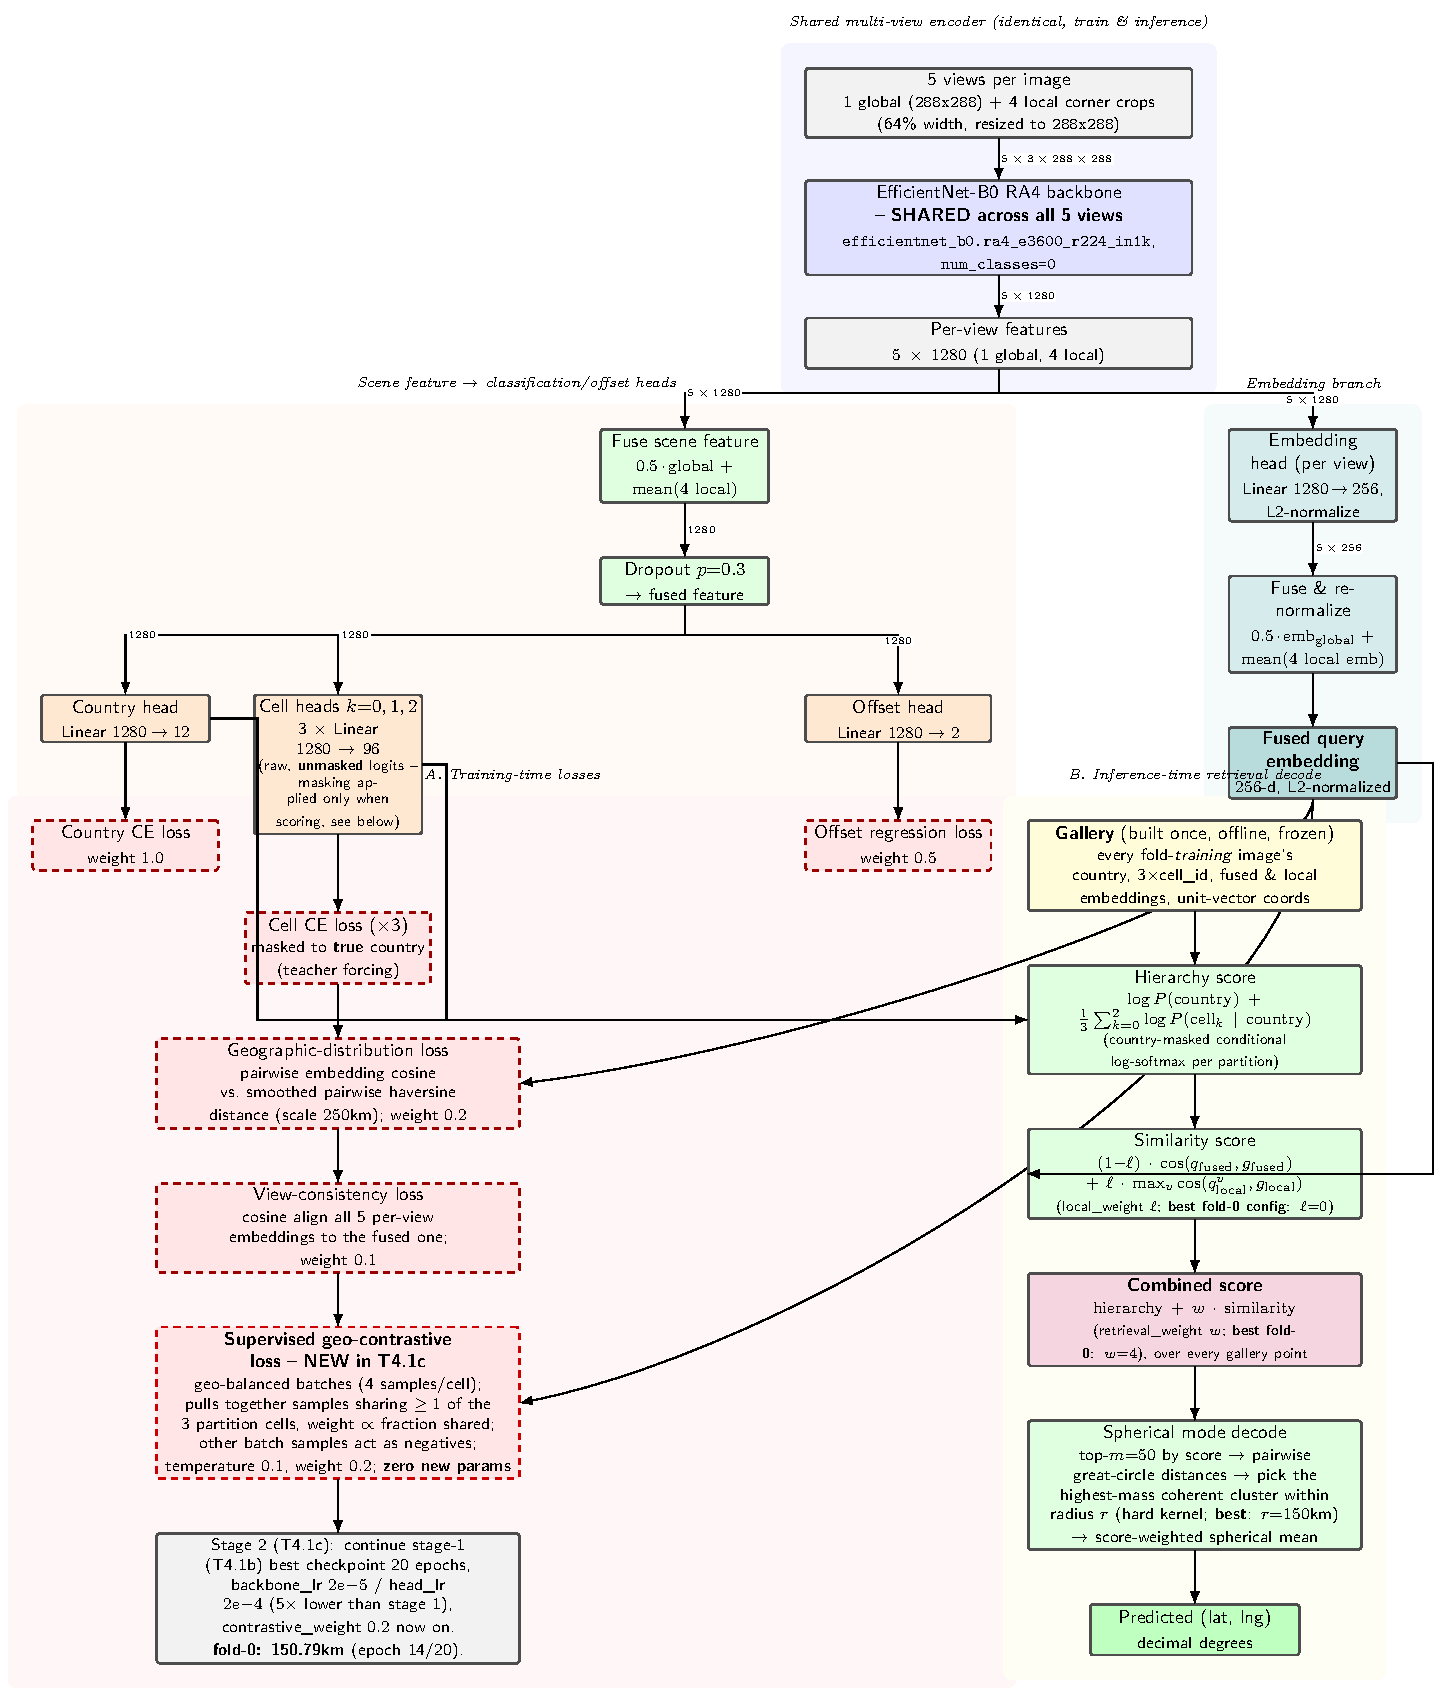
\includegraphics[width=0.98\textwidth]{figures/architecture_t4_1c.pdf}
\caption{Shared multi-view encoder, heads, training losses, and retrieval decode.}
\label{fig:arch}
\end{figure}

\section*{What was tried}
This was an iterative, evidence-driven search, not a single design.
\textbf{Backbones/architectures} (5-fold or fold-0 screens, honest fixed-decoder median km):
direct-regression MobileViT-XS (450--500km, badly underfit at low resolution) $\to$
hierarchical country+single-cell classifier with EfficientNet-B0 (193km) $\to$ K independent
coarse cell partitions combined at decode time instead of one finer partition, following
CPlaNet's argument that several coarse views triangulate a finer location without needing
enough data to populate a finer joint class space (183km at $K$=2, further gains through
$K$=3) $\to$ shared-backbone multi-view (global+4 local crops) retrieval against the full
training gallery with mode-aware spherical decoding (155km) $\to$ adding a supervised
geo-contrastive loss on top (\textbf{149.5$\pm$4.6km 5-fold CV, current best}). Backbone
swaps to FastViT-T8, RepViT and StarNet variants, and a MobileViT-XS run at 384px, all matched
or underperformed EfficientNet-B0 at 149--193km; $K$=4 partitions did not clearly beat $K$=3
either. A cross-architecture ensemble (blending this model's predictions with an earlier
direct classifier+offset model) was strictly worse than the retrieval model alone at every
blend weight -- the two models' errors were not complementary enough to help.

\textbf{Per-country error analysis} (5-fold, pooled, fixed decoder) was the most useful
diagnostic: median error splits sharply by country area/visual homogeneity, not by anything
architecture choices moved much:
\begin{center}
\begin{tabular}{lr@{\hspace{0.7em}}lr@{\hspace{0.7em}}lr}
\toprule
Country & km & Country & km & Country & km \\
\midrule
Iceland & 30 & Sweden & 125 & Turkey & 172 \\
Belarus & 68 & UK & 145 & Poland & 264 \\
Finland & 79 & & & Germany & 300 \\
Norway & 89 & & & Italy & 343 \\
& & & & Spain & 383, France & 404 \\
\bottomrule
\end{tabular}
\end{center}
France/Germany/Italy/Poland/Spain (42\% of the data) sit at 260--400km and did not move across
any of the 9 architecture variants tried -- large countries with visually similar
rural/suburban European road scenes are a real information ceiling at this model size and data
volume, not a tuning gap. Since the grading metric is the \emph{median}, and roughly half the
data already sits under 150km (Iceland/Belarus/Finland/Norway, all $<$90km), the only lever
that can move the aggregate median is Sweden/UK/Turkey, sitting just above the boundary.
\textbf{Targeted experiment}: upweighting the cell/country loss 3$\times$ for exactly those
three countries during a 25-epoch continued fine-tune. Result: Sweden improved (125$\to$102km)
and Turkey improved (172$\to$140km), but UK got worse (145$\to$167km) and untouched Norway/
Iceland regressed slightly (collateral damage from the reduced relative gradient share on
every other country) -- net effect on the fold was flat to slightly worse (154.9$\to$158.2km).
This was kept as a documented negative result rather than shipped. A 384px resolution
fine-tune (vs.\ the 288px trained resolution) was similarly inconclusive over 5 epochs (152--
157km, no trend distinct from noise) and was abandoned early rather than run to completion,
since it was not on track to beat the 288px baseline.

\section*{Final model and honest evaluation}
The submitted model uses the winning $K$=3, contrastive-loss recipe, warm-started from a
5-fold-CV checkpoint and then fine-tuned on \emph{all} labelled data (no held-out split, since
hyperparameters and epoch count were chosen from the separate CV screen above, not from this
run) so the final weights and gallery both see 100\% of the provided training images --
this is expected to be at least as good as the 149.5km CV estimate, since the CV models each
had to train and retrieve against only 80\% of the data. \textbf{Cross-validated headline
number: 150.6km median} (5-fold, pooled, single fixed decoder
config -- not per-fold cherry-picked), 447.5km mean, 55\% of images within 200km ("got the
city"), 82\% within 750km ("got the country").

\section*{Limitations and what we'd try with more budget}
The 5M-parameter ceiling forces a backbone (EfficientNet-B0, $\sim$4.0M feature-extractor
params) that is small relative to the visual variety of 12 countries; a larger backbone was
not legal, and none of the sub-5M backbones tried closed the France/Germany/Italy/Poland/
Spain gap. With more budget we would try: (1) a genuinely different decode-time prior -- a
uniform synthetic coordinate grid blended into the retrieval gallery, rather than only labelled
training points, to smooth the mode decoder's candidate density in sparsely-sampled regions of
large countries; (2) per-country-adaptive cell granularity (finer cells for compact, visually
distinctive countries where data density already supports it) rather than one global
MIN/MAX-cell-size policy; (3) a second, independently-seeded backbone under a stricter
per-branch parameter split, to get real ensemble diversity instead of the single-architecture
retrieval-vs-classifier blend that failed here.

\end{document}
